\documentclass[smallextended]{svjour3}       % onecolumn (second format)
\smartqed  % flush right qed marks, e.g. at end of proof
\usepackage{easy-todo}
\usepackage{mathptmx}      % use Times fonts if available on your TeX system
\usepackage{times}
\usepackage[utf8]{inputenc}
\usepackage{url}
\usepackage{tikz}
\usepackage{pgfplots}
\usepackage{latexsym}
\special{papersize=210mm,297mm} % to avoid having to use "-t a4" with dvips 
%\setlength\titlebox{6.5cm}  % You can expand the title box if you really have to
\usepackage{graphicx}
\usepackage{placeins}
\usepackage{framed}
\usepackage{pbox}
\usepackage{amsmath}
\usepackage{footnote}
\usepackage{supertabular}
\usepackage{algorithm} 
\usepackage{algpseudocode} 
\usepackage{caption}
\usepackage{gb4e}
\usepackage{natbib}

\pgfplotsset{compat=newest}

\let\proof\relax
\let\endproof\relax
\usepackage{amsthm}
\newtheoremstyle{break}
  {\topsep}{\topsep}%
  {\itshape}{}%
  {\bfseries}{}%
  {\newline}{}%
\theoremstyle{break}
\newtheorem{exmp}{Example}[section]

\DeclareMathOperator*{\argmin}{arg\,min}
\DeclareMathOperator*{\argmax}{arg\,max}

\title{Language-independent classifier-based modelling of source-side context information in Statistical Machine Translation}
\titlerunning{Source-side context in SMT}


\author{Maarten van Gompel \& Antal van den Bosch \\
  Centre for Language Studies \\
  Radboud University Nijmegen \\
  {\tt proycon@anaproy.nl}}
\authorrunning{van Gompel and van den Bosch}

%\date{}


\begin{document}
\maketitle

\begin{abstract} 
  We present a series of experiments focusing on the modelling of
  source-side context to improve Phrase-based Statistical Machine
  Translation. Statistical Machine Translation systems typically
  consist of a translation model and a language model. The former maps
  phrases in the source language to the target language, without
  regard for the context in which the source phrases occur. The latter
  models just the target language, and acts as a target-side model of
  context information after translation. We attempt to independently
  reproduce a line of existing research and test whether considering
  context information directly in the translation model has a positive
  effect on translation quality.  We furthermore investigate various
  ways discriminative classifier-based models can be integrated into
  Statical Machine Translation.  We will use proven techniques from
  Word Sense Disambiguation, effectively integrating these techniques in
  Statistical Machine Translation. Our approach is
  language-independent and knowledge-poor: we do not employ any
  explicit linguistic features computed by part-of-speech taggers,
  word sense disambiguation systems, supertaggers, or parsers, as used
  by previous work. We find only limited improvement of translation quality for
  certain formulaic corpora and conclude that explicit modelling of source-side
  context information does not add much to the data already implicitly
  available in the decode process.
\end{abstract}

\section{Introduction}

In phrase-based Statistical Machine Translation (SMT) the problem of
translating an input sentence from a source language to a target language is
implemented as a game of probabilities and a search for the most probable
translation option.  These probabilities are expressed in a number of models
that specialise in a certain aspect relevant to the translation process. The
``phrase-based'' characteristic is because phrases are the building blocks of
the translation model, generalising earlier approaches in
Statistical Machine Translation based on words.  Phrases in this
sense are sequences of one or more words, i.e. $n$-grams of variable
length (including unigrams). They are not constrained to form a
proper linguistic constituent of any kind.

Two models are at the core of phrase-based SMT: first there is the translation
model which maps the translation phrases in the source language ($S$) to
phrases in target language ($T$). Each mapping between phrases is associated
with a vector of probabilities, $p({phrase}_S|{phrase}_T)$ and
$p({phrase}_T|{phrase}_S)$. They can be seen to model the notion of
\emph{``semantic faithfulness''}; if a phrase is translated from one language
to another, the meaning should be preserved as accurately as possible.

The second core model is the language model. This model is monolingual
in nature and models the target language. It models what words are
likely to follow others and can be interpreted as modelling the
\emph{``syntactic fluency''} notion of translation; a translation should be
in a natural word order and be a typical sequence of words for the
target language.

A Machine Translation \emph{decoder} optimises a log-linear model of
these two, and additional other, models. Given an input sentence in
the source language, it searches through a vast space of all
``possible'' translation options, most nonsensical, for a path
maximising the probabilities according to each of the models, taking
into account different weights they may be assigned.

The study we currently present focusses on the role of additional
surface-form source-language context
information in the SMT process. The Language Model models context
for the target language. Yet in SMT there is no component modelling
context for the source language, whereas intuitively source-side context may
provide a powerful cue for translation. Consider the word ``bank'' and its
Spanish translation in examples~\ref{ex:bank1} and \ref{ex:bank2}.

\begin{exe} %gb4e package
\ex \textbf{English:} I don't trust the bank. \\
    \textbf{Spanish:} No me fio del banco.
\label{ex:bank1}

\ex \textbf{English:} The boat headed towards the bank of the river. \\
    \textbf{Spanish:} El barco se dirigió hacia la orilla del río.
\label{ex:bank2}
\end{exe}

The same English word, ``bank'', may express multiple semantic senses, some of
which are expressed by different words in Spanish. Source-side context
information may provide valuable clues to what sense is being employed, and
therefore what translation is correct.  The words ``boat'' and the phrase ``of
the river'' in example \ref{ex:bank2} provide clues that we are using
bank in its maritime sense. Example \ref{ex:bank1} is less obvious, but the
word ``trust'' could be seen to be a clue for ``bank'' denoting a
financial institution.

These examples are meant to illustrate the intuition that is behind our
research hypothesis. We hypothesise that the inclusion of source-side context
information in the translation model improves translation results, as the
context helps in providing a more accurate disambiguation. A counter-hypothesis
to this would be that although source-side context information is not modelled
explicitly, it is implicitly captured by the combination of translation model
and target language model, and explicit modelling has no added value.

There is an obvious overlap between what we aim to do here and the field of
Word Sense Disambiguation (WSD). We effectively test an integration of proven
techniques from WSD in Statistical Machine Translation, and apply these to
phrases rather than just words.

WSD systems often employ a variety of linguistic features. The focus of our
study, however, is to be independent of the explicit computation of
linguistically abstract features with language-dependent tools such as
lemmatisers, part-of-speech taggers, supertaggers, or dependency parsers
\cite{Rejwanul+11}. 
%We are interested only in the surface
%forms, the text as-is, and stay as close as possible to vanilla Phrase-Based
%Statistical Machine Translation, without using any language-specific external
%resources. 
In this fashion, we attempt to assess the merit of source-side
context information as purely as possible.

Not introducing extra data for the translation system means our goals have to
be set more modest as well. We may not expect the same gains as are achieved by
introducing extra data from linguistic preprocessors.

\section{Previous research}

The idea to integrate WSD approaches in SMT is not new, nor is the idea to use
source-side context information to disambiguate in translation. Various studies
have been conducted, offering mixed results. In the early days of SMT,
\cite{GarciaVarea+02} already explicitly modelled source-side context in a
maximum entropy model for word-based SMT, and report slightly improved error
rates on a translation task.

\cite{CarpuatWu05} were the first to directly tackle the question whether
full-scale WSD models were beneficial to translation quality when integrated in
SMT systems, and thus their work forms an important foundation for our own study.
Their approach uses an ensemble classification model that integrates
position-sensitive, syntactic, and local collocational features, which has
proven itself in competitive WSD tasks. This includes linguistic features such
as part-of-speech tags and lemmas, as well as more complex syntactic relations.
They test on a single Chinese--English test set only, and only
evaluate with BLEU,
which leaves open the question whether their conclusions would hold on
different language pairs, test sets, and using different evaluation metrics.
Their approach is word-based, however, and the level of integration is also limited.

Carpuat and Wu focus on the WSD model rather than on the SMT
model, whereas we place more focus on the SMT model and the
integration method, and keep our WSD model relatively
simple.

Despite their efforts, they reach the surprising conclusion that inclusion of
WSD techniques does \emph{not} yield better translation quality. Will these
results hold in a more modern Phrase-based Statistical Machine Translation
approach?

Two years later they expanded their study to full phrasal units
\citep{CarpuatWu07} and, for the first time, found results that did support the
hypothesis that SMT benefits from the integration of WSD techniques. They now
focus on better integration in \emph{phrase-based} SMT: ``Rather than using a
generic SenseEval model as we did in \cite{CarpuatWu05}, here both the WSD
training and the WSD predictions are integrated into the phrase-based SMT
framework.'' \citep{CarpuatWu07}. They also broaden their use of evaluation
metrics, yet still test on only Chinese to English.

The work of \cite{Gimenez+07}, from the same year, follows a similar
strategy. They use support vector machines to predict the phrase
translation probabilities for the phrase-translation table component
of SMT, rather than relying on the context-unaware Maximum Likehood
Estimate the statistical process produces. The feature vector for
their classifiers consists of both local context as well as global
context features.  In addition to the surface forms of the words, they
rely on shallow linguistic features such as part-of-speech tags and
lemmas. They conduct a manual evaluation judged on fluency and
adequacy, and conclude that considering context improves semantic
adequacy, yet does not benefit syntactic fluency. They remark that the
integration of the classifier probabilities in an SMT framework needs
further research, which is something that will indeed be a focus in
our present study.

The year 2007 saw a culmination of various studies integrating WSD techniques
in SMT using classifiers. A third study in this trend was \cite{Stroppa+07}.
They focus on the word form, as does this present study, and add only
part-of-speech features. On a dataset from the IWSLT 2006 challenge, for
Chinese--English and Italian--English, they achieve a significant improvement
for the former language pair, whereas the BLEU score for the latter language
pair fails to pass the significance test. We attempt to reproduce the
Chinese--English experiment in this study.

Source-context aware translation has also been attempted outside of the
predominant SMT framework. \cite{MBMT} implement a
simple form of example-based machine translation that is word-based and relies
chiefly on classifiers for the translation model component. Two studies derive
from the same concept while transcending a word-based paradigm:
\cite{MARKERBASED} use chunks delimited by common markers, and \cite{PBMBMT}
attempt a full extension to phrases similar to SMT. Although positive results
are achieved in the latter study, it does not rival state-of-the-art SMT.

The most important and complete study we build upon is
\cite{Rejwanul+11}, which in turn draws from the majority of the
aforementioned studies, and provides an extensive comparison between
them. Their study finds that including linguistically-informed
contextual features produces improvements, but not always; also,
different contextual features have different, unpredictable results,
some of which positive. The main contrast between our study and
theirs is that they focus on a variety of linguistically-informed
contextual features, whereas we depart from a language-independent
angle and intend to settle some of the conflicting reports whether
this may lead to an improvement in translation quality. A notable
focus in our study will be possible methods of integrating the
classifier probabilities in the SMT, as recommended also by
\cite{Gimenez+07}.


\section{Methodology}
\label{ref:methodology}

Like most of the previous work, we approach the machine translation
problem in a phrase-based fashion, which has superseded the simpler word-based
paradigm for quite some time. This means that phrases, defined as a
sequence of one or more words (that need not form a linguistic entity in any
way), form the basic building blocks of our translation model. The problem of
translating a sentence is decomposed into the problem of translating its phrasal
sub-parts and combining the results in the best order.

In describing our methodology, we first focus on the problem of phrasal
translation, adding in the source-side context component. This shall be done
using classifiers. Then we address how this can be integrated into a
phrase-based Statistical Machine Translation decoder, which also takes care of
the ordering aspect. 


\subsection{Modelling source-side context with classifiers}

In line with several previous studies \citep{Rejwanul+11,PBMBMT,
  Stroppa+07,MARKERBASED}, we make use of memory-based classifiers to
build a translation model informed by source-side context
information. More specifically, we will be using IB1 \citep{IB1}, an
implementation of $k$-Nearest Neighbour classification; IGTree
\citep{IGTree}, an optimised and lossless tree-based approximation
thereof; and TRIBL2, a mixture of IB1 and IGTree.

These algorithms are all implemented in the software package TiMBL
\citep{TIMBL}\footnote{\url{http://ilk.uvt.nl/timbl}} and are
well-suited for symbolic data and highly multivariate class spaces.
Moreover, memory-based classification has been a successful method in
the field of Word Sense Disambiguation \citep{SENSEVAL2,WSD2}.

When speaking of the $k$ nearest neighbours in the implementation of IB1,
IGTree and TRIBL2, we are actually referring to the neighbours at nearest
distance $k$. So even with $k=1$ we may be talking about multiple data points
that are all at equal distance.

%(these two paragraphs are paraphrased from my PBMBMT thesis, not sure to cite
%or prevent for risk of over-self-citation here)
% [Antal] that's no problem.
IGTree compresses the instance base into an ordered decision tree structure at
training time, and issues look-ups in this tree structure at test time. Unlike
other top-down induced decision tree methods such as C4.5, features in IGTree
are tested in a fixed order. This is computed only once 
for all features. This order is determined using metrics such as
\emph{information gain} or \emph{gain ratio}. They determine the relative
informativeness or disambiguating power of each feature and provide a ranking of
all features. 

IGTree's performance relies on the differences in information gain between
features. If these are small then IGTree may perform significantly below IB1
\citep{TIMBL}. A hybrid approach called TRIBL2 \citep{TIMBL} starts out with
IGTree and switches to a IB1 variant when a value mismatch occurs in the tree.
In this study, we therefore opt to use TRIBL2 over plain IGTree, but only when
using IB1 would have a prohibitively large impact on performance.

In our classifier-based translation model we model the probability
of a target phrase ($t$) given a source phrase ($s$) and context information
($C$). We can express this as $p(t|s,C)$.  \cite{Stroppa+07} state that
direct estimation of this probability using relative frequencies would result
in overestimation of large phrases, and that therefore a smoothing factor is
required. They proceed to say that through memory-based classification they
implicitly introduce precisely such a smoothing factor implicitly.

Given a source phrase and context information, the classifier yields classes
corresponding to target phrases, with an associated weight. After
normalization, these can be considered a posterior distribution of
target phrases. 

We primarily focus on the modelling of local context, i.e. words in the
immediate vicinity of the source phrase. Take $w_0$ to be the first word of
the source phrase $s$, then for a local context size of $n$ words to the left and
$m$ to the right we construct the feature vector $C$ as
follows\footnote{For context words out of the sentence's bounds, placeholders
are used instead}:

\begin{equation}
  C = \langle w_{-n} .. w_{-1} , s , w_{|s|+1} .. w_{|s|+m} \rangle
\end{equation}

Now there are two ways in which we can construct a classifier:

\begin{itemize}
  \item \textbf{Monolithic classifier} -- One aggregated classifier for all
    source phrases.
  \item \textbf{Classifier experts} -- One classifier per source phrase.
\end{itemize}

In this study we will use and compare both methods, which is, for the task at
hand, the first such a comparison in the literature as far as we know.

For the monolithic classifier, the first feature in the ranking will always be
$s$. Nevertheless, it is quite conceivable that a match for the context is not
found and the classifier proceeds to match on another feature. To prevent
situations in which the classifier falls back to a completely different source
phrase, and thus comes up with unrelated translation options, we enforce that
the source phrases need to match, which is what \cite{Stroppa+07} do as
well.

For the classifier experts, on the other hand, the source
phrase carries no discriminative power, as it is shared amongst all instances. We
therefore omit it from the feature vector.

\subsection{Training}

The translation model is trained on parallel corpus data. We follow a common
MT pipeline, and additionally derive classifier training data from the data.

Given a tokenised and sentence-aligned parallel corpus, we iteratively learn
word alignments using GIZA++ \citep{GIZA}. Then we identify and extract phrase
pairs using the {\em grow-diag-final}\/ algorithm \citep{OchNey2003}. The
result is a phrase-translation table mapping source phrases to target
phrases, along with associated scores which we will discuss in the next
section. %This phrase-translation table effectively constitutes the translation
%model.

The translation model would be finished if we would want to leave it to be
non-context-informed. We have some additional steps to perform to train our
context-informed classifiers. We take the phrase-translation table, along with
the parallel corpus, as a basis for extracting training instances.

We build indexed pattern models of all source phrases and target
phrases that occur on their respective side the parallel corpus, and
which also occur in the phrase-translation table. An indexed pattern
model maps each distinct phrase to the locations in the corpus where
it occurs.  Additionally, a reverse index is included in the model for
the target-side of the corpus, which maps any given
$(sentence, token)$ position to a set phrases that begins at that
position.  This is computed using the software package
\emph{colibri-core},\footnote{\url{http://proycon.github.io/colibri-core}}
which takes care of a losslessly compressed in-memory representation
for all phrases, and allows us to cope with large corpora. Given these
two pattern models $M_{source}$ and $M_{target}$ we can quickly and
efficiently extract the context for each phrase pair, as shown in
simplified form in Algorithm~\ref{alg:featureextract}.

\begin{algorithm}
\caption{Algorithm for feature extraction for training classifiers.  Take $n$
again to be the left context, $m$ to be the size of the right context, and
$w{(i,j)}$ to denote the word in the source corpus in sentence $i$, token $j$.
The vector $C$ represents the context information and constitutes the feature
vector.  The algorithm will return a list containing two-tuples $(C,t)$.  }
\label{alg:featureextract}
\begin{algorithmic}
\State instances $\gets []$
\For {$(s \in M_{\text{source}}, t \in M_{\text{target}})$}
  \For {$i \in (M_{\text{source}}[s] \cap M_{\text{target}}[t])$}
    \For{$j \in M_{\text{source}}[s][i]$}
        \State $C \gets \langle w_{i,j-n} \ldots w_{i,j-1}, s, w_{i,j+|s|+1} \ldots w_{i,j+|s|+m} \rangle$
        \State \Call{instances.append}{$(C, t)$} 
      \EndFor
  \EndFor
\EndFor \\
\Return{instances}
\end{algorithmic}
\end{algorithm}
    
\noindent
This algorithm is implemented in \emph{colibri-mt}.
\footnote{\url{https://github.com/proycon/colibri-mt}}

The returned instances can be stored directly, either in a single model for the
monolithic approach or in separate models for each $s$ for the classifier
expert approach. A final training phase then computes the feature ranking and
transforms this data into the instance base format required for TiMBL.

%When extra training data for the classifier(s), 
It may well happen that either 1) an $(s,t)$ pair only occurs once, or
2) a pattern $s$ occurs in multiple contexts but all map to the same
$t$. In such cases, a context-informed classifier has no added value
and therefore such instances are omitted from the training data.

\subsection{Integration in an SMT Decoder}
\label{sec:smtintegration}

The task of an SMT decoder is to find the best translation among a pool
of possible translation hypotheses. The best translation hypothesis is the
translation hypothesis that maximises a log-linear combination and is sought
after in a beam-search algorithm. This log-linear combination draws from
various models, such as a translation model (i.e. the phrase-translation
table), a target-language model, and optionally additional models such as a
distortion model and a word-reordering model. 

The SMT model is generally expressed as in Equation~\ref{eq:smtmodel}, taking
sentence $e$ to be the translation in the target language, and $f$ to be the sentence to be
translated, in the source language.

\begin{equation}
\argmax_e p(e|f) = \argmax_e p(f|e)p(e)
\label{eq:smtmodel}
\end{equation}

Bayes' rule inverts the problem into two factors\footnote{The denominator p(f)
can be dropped as it would not alter the outcome of the \emph{argmax}
function}, the former corresponding to the translation model, and the latter
corresponding to the language model. 

The translation model is a mapping of the set of source phrases ($S$) to the
set of target phrases ($T$). Each phrase pair $(s,t)$ where $s \in S$ and $t
\in T$ is described by a score vector indicating the likelihood of
translation. This score vector most notably consists of the probabilities
$p(s|t)$ and $p(t|s)$. In addition, the lexical weighting probabilities $lex(s|t)$
and $lex(t|s)$ express the probability of a phrase pair word-by-word, and are
often included as components in the score vector. During decoding, the total
score of the translation model and other models is expressed as a log-linear
combination, in which different weights can be assigned to each of the
components of the score vector. These weights are hyperparameters to the task and
are typically optimised automatically on development data using for instance
Minimum Error Rate Reduction \citep{MERT}.

The probability $p(t|s)$ is the one we are interested in. Recall that the
classifiers seek to model $p(t|s,C)$, where $C$ constitutes the vector of
context information. The hypothesis under investigation in the present study is
that $p(t|s,C)$ is a more accurate measure than $p(t|s)$.

The state-of-the-art SMT decoder used in the majority of MT studies is Moses
\citep{MOSES}. Moses offers no facilities to take source-side context
information in account. We had to consider three options to achieve our goal of
integrating source-side context: 1) creating a new decoder; 2) enhancing
Moses; or 3) using a bypass method. Although we initially set out to create a
new decoder, it proved to be too difficult to attain the same quality as Moses.
We therefore decided, in line also with most of the literature, to follow the
third option and use a bypass method; this allows us to use Moses as a black box.

The bypass method is a \emph{discriminative translation filtering}
step \citep{Rejwanul+11}. It performs context-aware classification in
a pre-processing step, namely through alteration of the
phrase-translation table, and bypasses the need to alter the
decoder. Taking each sentence individually, we ensure that the entries
in the phrase-translation table are explicitly tuned to the
source-side context. The output of the classifier(s) acts as the
filter and constrains the translations options, as well as adjusts the
score vector. Each instance of a source phrase receives a separate entry
in the phrase-translation table, as opposed to one source phrase
applying to all instances in the test data.

To achieve this, each source phrase in the phrase-translation table is
replaced by a representation of its position in the test data, e.g.
$(1,0)$ for first sentence, first word.  This is done using the
software package \emph{colibri-mt}. It creates an indexed pattern
model on the test data, constrained by the phrases in the
phrase-translation table. This thus constitutes a mapping of all
distinct source phrases in the phrase-translation table to the indices
in the test corpus that are instances of these phrases.

Subsequently we invoke the classifier(s) and construct the altered
phrase-translation table as shown in Algorithm~\ref{alg:contextmoses}.

\begin{algorithm}
\begin{algorithmic}
  \For {$s \in M_{\text{test}}$}
  \For {$(i,j) \in M_{\text{test}}[s]$}
    \State $C \gets \langle w_{i,j-n} \ldots w_{i,j-1}, s, w_{i,j+|s|+1} \ldots w_{i,j+|s|+m} \rangle$
    \State $[(t, p(t|s,C) )] \gets$ \Call{classify}{$s,i,j,C$}
    \State {\Call {appendtophrasetable}{$s,i,j,[(t, p(t|s,C)]$}}
  \EndFor
\EndFor
\end{algorithmic}
\caption{Classifier invocation on test data. Take $M{\footnotesize\text{test}}$ to be the pattern
model of the test data, i.e. a map of source phrases occuring in the test
data, and $[(t,p(t|s,C))]$ to be a list of translation options ($t$) with
associated probability $p(t|s,C)$.}
\label{alg:contextmoses}
\end{algorithm}

In Algorithm~\ref{alg:contextmoses} we examine each source phrase in turn, find
where it occurs in the test data ($i,j$) using the pattern model
($M_{\text{test}}$), and extract context information ($C$). The context
information constitutes our feature vector, with which we invoke the
appropriate classifier. This is either the monolithic classifier, or the
classifier expert pertaining to the source phrase under consideration. The
result of this classification is a distribution of translation options for that
source phrase in the given context, along with a classifier score for each
option. After normalisation, this score is $p(t|s,C)$. We now have two score
weighting methods for integrating this in the score vector for the phrase pair:

\begin{itemize}
  \item \textbf{Replace} - Replace the $p(t|s)$ probability with $p(t|s,C)$;
  \item \textbf{Append} - Leave the existing $p(t|s)$ as it was, and append
    $p(t|s,C)$ as a new score to the score vector.
\end{itemize}

The score weighting of choice is applied and the data is entered into the
altered phrase-translation table. The source phrase takes the form of a
sequence of $(i,j)$ indices, rather than the actual words. The test data is
replaced with a series of consecutive positions as well. These two altered data
sets are now the input to Moses, which can now run unmodified. 

\section{Experiments}

We conduct a large number of experiments to assess whether integration of
context-informed classifiers in Statistical Machine Translation leads to
an improvement in translation quality. 


\subsection{Data sets}

For the translation model, we rely on a parallel corpus as our main source of
input. Whenever the source is untokenised, we tokenise the data using
\emph{ucto}.\footnote{An open-source regular-expression based tokeniser with
unicode support, \url{http://ilk.uvt.nl/ucto}} For the language model, we
simply reuse the target-side portion of the parallel corpus; we do not
introduce additional data for the language model in our experiments.

We use various corpora\footnote{Europarl, EMEA and JRC-Acquis can be obtained through
\url{http://opus.lingfil.uu.se/}} and test various language pairs as we hope to
come to a general conclusion. Table~\ref{tab:datasets} lists them all, along with the amount of
sentence pairs we used for training, development and testing.

\begin{table}
\begin{center}
\begin{tabular}{lrr}
& \textbf{Languages} & \textbf{Sentence Pairs} \\
\hline
\multicolumn{3}{l}{\pbox{12cm}{\textbf{Europarl} -- \emph{The proceedings of the
European Parliament} \citep{EUROPARL,OPUS2012}} } \\
& English to Spanish & $250,000$ / $2000$ / $2000$ \\
& English to Dutch & $250,000$ / $5000$ / $5000$ \\
\multicolumn{3}{l}{\textbf{EMEA} -- \emph{Documents of the European Medicines
Agency} \citep{OPUS2012} } \\
 & Spanish to English & $1,088,333$ / $5000$ / $5000$ \\
 & English to Dutch & $1,080,894$ / $5000$ / $5000$ \\
\multicolumn{3}{l}{\pbox{12cm}{\textbf{Fryske Akademy Parallel Corpus} -
\emph{A collection of texts in
Frisian and Dutch, contains numerous books and other sources} \citep{OERSETTER}
\footnote{This corpus is not publicly available unfortunately} } } \\
 & Dutch to Frisian & $137,937$ / $2000$ / $2000$ \\
 & Frisian to Dutch & $137,937$ / $2000$ / $2000$ \\
\multicolumn{3}{l}{\textbf{JRC-Acquis} - \emph{A collection of legislative documents of the
European Union} \citep{OPUS2012} } \\
 & English to Spanish & $1,233,670$ / $5000$ / $5000$ \\
 & English to Spanish & $250,000$ / $5000$ / $5000$ \\
\multicolumn{3}{l}{\pbox{12cm}{\textbf{IWLST 2012 TED Talks} - \emph{Transcripts and translations of TED
talks, used for subtitling, as used in the IWSLT 2012 Evaluation Campaign}
    \citep{WIT3,IWSLT12} } } \\
 & English to Dutch & $127,806$ / $885$ / $1569$ \\
\multicolumn{3}{l}{\pbox{12cm}{\textbf{IWLST 2006 Evaluation Campaign} -
\emph{Collection of phrases from a phrasebook / traveller's guide } } } \\
 & Chinese to English & $40,274$ / $489$ / $486$ \\
 \multicolumn{3}{l}{\pbox{12cm}{\textbf{Yandex 1M Web Corpus}  -
 \emph{Phrases crawled from the web by Russian search engine Yandex} } } \\
 & English to Russian & $990,000$ / $5000$ / $5000$ \\
\end{tabular}
\caption{Overview of parallel corpora used for experiments. The three values
for sentence pairs correspond to the size of the training, development and test
set, respectively.}
\label{tab:datasets}
\end{center}
\end{table}

\todo{TODO: add torrent link}

% goed plan, die academic torrents?

\subsection{Evaluation}

We assess translation quality along five widely-used automated metrics,
as human evaluation is prohibitively expensive:

\begin{enumerate} %paraphrased from PBMBMT thesis
\item \textbf{BLEU} - BLEU \citep{BLEU} is probably the most widely-used metric
in Machine Translation. It computes a weighted average of $n$-gram overlap
between the system output and reference output. The score thus increases as
more $n$-grams in the reference translation are found in the system output.
\item \textbf{NIST} - NIST intends to improve upon BLEU. It takes into account
how informative a particular $n$-gram is by assigning more weight to rare
$n$-grams and less to highly-frequent $n$-grams.  
\item \textbf{METEOR} - METEOR \citep{METEOR} also attempts to improve upon
  BLEU and attempts to emulate human judgement better. Unlike the prior
  metrics, it places emphasis on recall rather than precision.
\item \textbf{Word-Error Rate (WER)} - This is a simple metric derived from the
minimum edit-distance, i.e. Levenshtein, algorithm. It counts the number of
substitutions, insertions and deletions necessary to transform the translation
into the reference sentence, with words as the basic unit. The lower
the score, the more similar the translation is to the reference.  
\item \textbf{Position Independent Word Error Rate (PER)} - This is a variant of the
metric above, but here the order of the words is not taken into account. Any
ordering of the same words will have the same score. The lower the score, the
more similar the translation is to the reference.
\end{enumerate}

For each experiment we construct a non-context-informed baseline. This
baseline does make use of our full pipeline, i.e. the bypass method described
in Section~\ref{sec:smtintegration}, but it does not invoke the
classifiers.  We do this to ensure the only difference is the actual
integration of context information, and that differences in result can not be
attributed to minor idiosyncrasies of the implementation.

We test statistical significance of our systems on the BLEU score, compared to
the non-context informed baseline For this we use pairwise bootstrap sampling
\citep{KoehnStatSig} with $5000$ iterations. Statistical significance at
$p<0.05$ will be marked with an asterisk in the results.

\subsection{Parameter optimisation}
\label{sec:paropt}

An SMT system relies heavily on parameter optimisation. Each component of the
score vector is weighted by a separate parameter. These parameters are
experimentally determined on development data using Minimum Error Rate
Reduction \citep{MERT}, in which we optimise on the BLEU score. MERT is,
however, known to have high variance across multiple runs, due to many local
optima in the search space. We therefore do not run MERT independently on each
experimental run, but only on the baseline run, and use those weights for
subsequent runs using the replace method.\footnote{The append method would
require an extra weight that the baseline does not have} Again, the motivation
here is to keep all variables equal except for the integration of context
information, so we can make a fair assessment.

%talk about parameter optimisation in classifier
While we conduct parameter optimisation for the parameters of the SMT
decoder, we do not do so for the classifiers. Yet, these too could
be optimised. This is only feasible for the classifier experts; recall
that the monolithic classifier necessarily has extra constraints
imposed on it to prevent translations that do not occur in the
phrase-translation table. This has the disadvantage of making it hard
to run standard parameter optimisation algorithms.

Optimisation of classifier parameters comes with a number of challenges.
Ideally, it should not be independent of the optimisation of the decoder
parameters, and the classifier parameters should be evaluated on the
end result, i.e. the full sentential translations, according to one or more MT
metrics. This, however, is prohibitively expensive as it vastly increases the
parameter search space and thus the complexity of the problem. As a concession
for the sake of computability, classifier parameter optimisation can be considered
independently and assessed through simpler cross-validation or leave-one-out
methods (depending on the number of instances in the classifier expert).  This
still introduces a significant computational bottleneck.  

Optimisation can be taken a step further by also optimising the local context
size, i.e. the make up of the feature vector, on a by-classifier basis, as
opposed to using the same context size for all classifiers. This has been
extensively researched in \cite{WSD2} in the context of cross-lingual Word
Sense Disambiguation, rather than full Machine Translation. In this study,
classifier parameter optimisation showed an overall negative effect, most
likely due to overfitting, especially when combined with variable context
selection. Variable context selection by itself did make a small positive
impact.

Given the results of this prior study, and due to the inherent computational
complexity of different layers of optimisation (even under an independence
assumption) we choose to limit ourselves to just optimisation of the SMT
decoder parameters in this study. These parameters have the most immediate and
largest impact as they are directly optimised on the evaluation metric used.
Note that although we forego on explicit variable context selection, an
implicit form is still there for the classifier experts; the feature weights
are computed on a by-classifier basis.

\section{Results}

In this section we will present the results of our experiments.
Our largest issue with the present MT literature on this subject is that we too often
see that hypotheses are tested only on or two corpora, with just one or two
language-pairs. We feel that from such results, generic conclusions are too
quickly drawn. To prevent this pitfall, our experiments are distributed amongst
various corpora and language pairs.

Section~\ref{sec:results1} will focus on our main hypothesis; does inclusion
of surface-form source-side-context lead to improved translation quality? We
will soon observe that this question is not straightforward to answer, as
the different corpora and language pairs often paint a conflicting image. We
posit a number of hypotheses to determine in which cases source-side-context
might work. Section~\ref{sec:qqthreshold} investigates whether a certain
criticial mass of translation quality or quantity of training material is needed
before source-side context can make an impact. Section~\ref{sec:morphdir}
analyzes whether translation from morphologically simpler to more complex
language is what makes the difference. Section~\ref{sec:quantanal} conducts
a quantitative analysis to assess whether the classifiers make an impact even
if this does not reflect in the translation quality.

Our secondary hypotheses concern the ways in which classifiers can be
integrated in SMT, here we investigate the impact of the classifier type and
weighting methods.  These are assessed in sections~\ref{sec:typeopt} and
\ref{sec:weighting}, respectively. We conclude the result section with a
qualitative analysis in Section~\ref{sec:qualanal}.

\subsection{Source-side context vs. no context}
\label{sec:results1}

The primary objective of our study is to assess the role of
source-side context information. To this end we conducted a series of
experiments on various corpora and language pairs. The first results,
on the IWSLT 2006 Evaluation Campaign, Chinese to English, are listed
in Table~\ref{tab:iwslt2006zhen}. They show a consistent advantage of
having the source-side classifiers. A dataset from the same source
\footnote{This dataset is not publicly available. As we do not have the exact set used by
  \cite{Stroppa+07}, we have to assume our training and test sets,
  whilst drawn from the same source, are distinct subsets from the
  ones used by \cite{Stroppa+07}.} was used in \cite{Stroppa+07}, who
also reported positive results.

\begin{savenotes}
\begin{table}
\begin{center}
\begin{tabular}{|l|ccccc|}
\hline
\textbf{System} & \textsc{BLEU}  & \textsc{METEOR}  & \textsc{NIST}  & \textsc{WER}  & \textsc{PER}  \\ 
\hline
\multicolumn{6}{|c|}{IWSLT 2006 -- Chinese$\rightarrow$English} \\
\hline
Baseline (replace/M/opt) & 0.2877 & 0.532 & 5.3809 & 57.33 & 47.66 \\ 
%l1r1 vs baseline: System 1 BLEU better: 4908 / 5000 = 0.9816 -- BLEU SIGNIFICANT at p = 0.05
l1r1 (monolithic/replace/opt/tribl2) & 0.2959$*$ \footnote{Statistically
significant compared to the baseline at $p<0.05$} & 0.5306 & 5.5294 & 55.69 & 46.41 \\
%System 1 BLEU better: 4957 / 5000 = 0.9914 -- BLEU SIGNIFICANT at p = 0.05
l1r1 (experts/replace/opt/ib1) & 0.2978$*$ & \textbf{0.5339} & 5.5313 & 55.66 & 46.33 \\ 
%System 1 BLEU better: 4781 / 5000 = 0.9562 -- BLEU SIGNIFICANT at p = 0.05
l2r1 (monolithic/replace/opt/tribl2) & 0.2941$*$ & 0.5305 & 5.5192 & 55.29 & 46.23 \\ 
%System 1 BLEU better: 4847 / 5000 = 0.9694 -- BLEU SIGNIFICANT at p = 0.0
l2r1 (experts/replace/opt/ib1) & 0.2955$*$ & 0.5338 & 5.5391 & 55.53 & 46.23 \\ 
%System 1 BLEU better: 4941 / 5000 = 0.9882 -- BLEU SIGNIFICANT at p = 0.05
l2r2 (monolithic/replace/opt/tribl2) & 0.2968$*$ & 0.5281 & \textbf{5.5493} & \textbf{55.10} & \textbf{46.09} \\ 
l2r2 (experts/replace/opt/ib1) & \textbf{0.2986}$*$ & 0.5304 & 5.5467 & 55.47 & 46.36 \\ 
l3r3 (monolithic/replace/opt/tribl2) & 0.2962$*$ & 0.5275 & 5.5364 & 55.26 & 46.36 \\ 
l3r3 (experts/replace/opt/ib1) & 0.2950$*$ & 0.5328 & 5.5433 & 55.66 & 46.41 \\ 
\hline
\end{tabular}
\caption{Results for Chinese to English on IWSLT 2006 Evaluation Campaign data.
The numbers in the context-aware configurations (l$x$r$y$), refer to the size
of the left respectively right context.}
\label{tab:iwslt2006zhen}
\end{center}
\end{table}
\end{savenotes}

Several local context sizes have been attempted. The number after \texttt{l}
refers to the numbers of words to the left of the source phrase. The number
after \texttt{r} denotes the right context size. Further parameters to the
system are enclosed within parentheses.  Recall that the classifiers may be
built in two distinct ways, a single \emph{monolithic} configuration (with
\emph{tribl2}), as is used here, or a classifier \emph{expert} configuration
(with \emph{ib1}).  Secondly, score weighting can be done either through the
\emph{replace} or the \emph{append} method. In this experiment, only the former
was used.  In this section we focus exclusively on the question whether
context-informed systems are beneficial, and if so, with what context size; a
comparison of the score weighting methods and classifier configurations is
postponed until a later section.  For the current and most of our experiments,
weights to the SMT decoder have been optimised (\emph{opt}) using MERT, on the
baseline.

For this experiment we draw the conclusion that the integration of
source-side context-informed classifiers may indeed be beneficial.
The highest results are attained with a configuration of two words to
the left and two words to the right, but the results from the various
context configurations are fairly close. 
%It is likely that using
%different data results in a different ranking.

This positive conclusion, however, can not be easily generalised.
Table~\ref{tab:europarl250k}, for example, presents a more scattered image,
with results primarily below baseline. This experiment was conducted on 250,000
training instances of the Europarl corpus, from Dutch to
English.

\begin{table}
\begin{center}
\begin{tabular}{|l|ccccc|}
\hline
\textbf{System} & \textsc{BLEU}  & \textsc{METEOR}  & \textsc{NIST}  & \textsc{WER}  & \textsc{PER}  \\ 
\hline
\multicolumn{6}{|c|}{europarl250k-nl-en} \\
\hline 
Baseline (replace/M/opt) & \textbf{0.2801} & \textbf{0.5181} & 7.4274 & 63.40 & 45.0 \\ 
l1r1 (monolithic/replace/opt/tribl2) & \textbf{0.2801} & \textbf{0.5181} & 7.4274 & 63.40 & 45.0 \\ 
l2r1 (monolithic/replace/opt/tribl2) & 0.2713 & 0.509 & 7.4168 & 63.08 & 45.01 \\ 
l2r1 (experts/replace/opt/ib1) & 0.2722 & 0.5105 & \textbf{7.4344} & 63.05 & \textbf{44.94} \\ 
l2r2 (monolithic/replace/opt/tribl2) & 0.2696 & 0.5078 & 7.4025 & 63.18 & 45.07 \\ 
l2r2 (experts/replace/opt/ib1) & 0.271 & 0.5095 & 7.423 & \textbf{63.04} & 44.98 \\ 
l3r3 (monolithic/replace/opt/tribl2) & 0.2673 & 0.5061 & 7.3826 & 63.29 & 45.16 \\ 
l3r3 (experts/replace/opt/ib1) & 0.268 & 0.5069 & 7.3879 & 63.18 & 45.1 \\ 
\hline
\end{tabular}
\caption{Results on Europarl 250k, Dutch to English}
\label{tab:europarl250k}
\end{center}
\end{table}

In Table~\ref{tab:iwslt2012} we see results on the IWSLT 2012 corpus, for the
same language pair, which paints a similar picture, albeit closer to the
baseline.

\begin{savenotes}
\begin{table}
\begin{center}
\begin{tabular}{|l|ccccc|}
\hline
\textbf{System} & \textsc{BLEU}  & \textsc{METEOR}  & \textsc{NIST}  & \textsc{WER}  & \textsc{PER}  \\ 
\hline
\multicolumn{6}{|c|}{IWSLT 2012 -- Dutch$\rightarrow$English} \\
\hline 
\hline 
Baseline (replace/M/opt) & 0.3014 & \textbf{0.5577} & 7.2676 & 52.91 & 39.98 \\ 
l1r1 (monolithic/replace/opt/tribl2) & 0.3008 & 0.5526 & 7.3201 & 52.17 & 39.57 \\ 
%System 1 BLEU better: 2894 / 5000 = 0.5788
l1r1 (experts/replace/opt/ib1) & \textbf{0.3018}$\dagger$\footnote{Score is
\emph{not} significant at $p<0.05$.} & 0.5536 & 7.3195 & 52.23 & 39.52 \\ 
l2r1 (monolithic/replace/opt/tribl2) & 0.2997 & 0.5521 & 7.3253 & 52.1 & 39.48 \\ 
l2r1 (experts/replace/opt/ib1) & 0.3007 & 0.5532 & 7.3286 & 52.14 & 39.5 \\ 
l2r2 (monolithic/replace/opt/tribl2) & 0.3000 & 0.5516 & 7.3303 & 51.99 & 39.49 \\ 
l2r2 (experts/replace/opt/ib1) & 0.3009 & 0.5529 & \textbf{7.3355} & 51.98 & \textbf{39.44} \\ 
l3r3 (monolithic/replace/opt/tribl2) & 0.2994 & 0.5497 & 7.3264 & \textbf{51.92} & 39.57 \\ 
l3r3 (experts/replace/opt/ib1) & 0.2995 & 0.5498 & 7.3243 & 51.96 & 39.57 \\ 
\hline
\end{tabular}
\caption{Results on IWSLT 2012, Dutch to English}
\label{tab:iwslt2012}
\end{center}
\end{table}
\end{savenotes}

We observe a high degree of variability between our various experiments.
Conclusions drawn from one dataset cannot be generalised.
Further experiments in this section will underline this observation. 

The EMEA corpus (Table~\ref{tab:emea}) shows the most positive results. The JRC
Acquis corpus (Table~\ref{tab:jrc250k}) also shows positive results, although by a small
margin. Both experiments were done for English to Spanish, and an English to
Dutch experiment was added for EMEA, on which the results also hold. In these
experiments we did not conduct parameter optimisation; we instead used a
uniform (uni) distribution of weights for the translation model, and similar
defaults for the other components.

\begin{table}
\begin{center}
\begin{tabular}{|l|ccccc|}
\hline
\textbf{System} & \textsc{BLEU}  & \textsc{METEOR}  & \textsc{NIST}  & \textsc{WER}  & \textsc{PER}  \\ 
\hline
\multicolumn{6}{|c|}{EMEA-en-es} \\
\hline
Baseline (replace/M/uni) & 0.6771 & 0.7617 & 12.0214 & 30.87 & 24.23 \\ 
%System 1 BLEU better: 5000 / 5000 = 1 -- BLEU SIGNIFICANT at p = 0.05
l1r1 (monolithic/replace/uni/tribl2) & \textbf{0.6935}$*$ & \textbf{0.7726} & \textbf{12.3003} & \textbf{29.39} & \textbf{22.97} \\ 
%System 1 BLEU better: 5000 / 5000 = 1 -- BLEU SIGNIFICANT at p = 0.05
l1r1 (experts/replace/uni/ib1) & 0.6895$*$ & 0.7698 & 12.2273 & 29.76 & 23.34 \\ 
\hline 
Baseline (append/M/uni) & 0.6826 & 0.7651 & 12.1423 & 30.10 & 23.64 \\ 
%System 1 BLEU better: 5000 / 5000 = 1 -- BLEU SIGNIFICANT at p = 0.05
l1r1 (monolithic/append/uni/tribl2) & \textbf{0.6973}$*$ & \textbf{0.7747} & \textbf{12.3746} & \textbf{28.77} & \textbf{22.58} \\ 
%System 1 BLEU better: 5000 / 5000 = 1 -- BLEU SIGNIFICANT at p = 0.05
l1r1 (experts/append/uni/ib1) & 0.6938$*$ & 0.7723 & 12.317 & 29.13 & 22.85 \\ 
\hline
\multicolumn{6}{|c|}{EMEA-en-nl} \\
\hline
Baseline (replace/M/uni) & 0.6612 & 0.7502 & 11.5287 & 32.77 & 26.22 \\ 
%System 1 BLEU better: 5000 / 5000 = 1 -- BLEU SIGNIFICANT at p = 0.05
l1r1 (monolithic/replace/uni/tribl2) & \textbf{0.6725}$*$ & \textbf{0.7572} & \textbf{11.7539} & \textbf{31.62} & \textbf{25.27} \\ 
%System 1 BLEU better: 5000 / 5000 = 1 -- BLEU SIGNIFICANT at p = 0.05
l1r1 (experts/replace/uni/ib1) & 0.6697$*$ & 0.7552 & 11.7028 & 31.88 & 25.52 \\ 
\hline 
Baseline (append/M/uni) & 0.6646 & 0.7525 & 11.6214 & 32.27 & 25.81 \\ 
%System 1 BLEU better: 5000 / 5000 = 1 -- BLEU SIGNIFICANT at p = 0.05
l1r1 (monolithic/append/uni/tribl2) & \textbf{0.6743}$*$ & \textbf{0.7587} & \textbf{11.8008} & \textbf{31.38} & \textbf{25.07} \\ 
%System 1 BLEU better: 5000 / 5000 = 1 -- BLEU SIGNIFICANT at p = 0.05
l1r1 (experts/append/uni/ib1) & 0.6718$*$ & 0.7567 & 11.7539 & 31.60 & 25.32 \\ 
\hline
\end{tabular}
\caption{Results on EMEA, English to Spanish and English to Dutch}
\label{tab:emea}
\end{center}
\end{table}



\begin{savenotes}
\begin{table}
\begin{center}
\begin{tabular}{|l|ccccc|}
\hline
\textbf{System} & \textsc{BLEU}  & \textsc{METEOR}  & \textsc{NIST}  & \textsc{WER}  & \textsc{PER}  \\ 
\hline
\multicolumn{6}{|c|}{JRC250k-en-es (sample 1)} \\
\hline 
Baseline (replace/M/uni) & 0.4510 & 0.6241 & 9.6386 & 47.02 & 31.41 \\ 

l1r1 (monolithic/replace/uni/tribl2) & 0.4503 & 0.6240 & \textbf{9.7726} & \textbf{46.25} & \textbf{30.88} \\ 
l1r1 (experts/replace/uni/ib1) & \textbf{0.4513}$\dagger$\footnote{Score is
\emph{not} significant at $p<0.05$.} & \textbf{0.6243} & 9.7619 & 46.31 & 30.91 \\ 
\hline 
Baseline (append/M/uni) & 0.4526 & 0.6242 & 9.8183 & 45.82 & 30.78 \\ 
l1r1 (monolithic/append/uni/tribl2) & 0.4513 & 0.6237 & 9.8741 & 45.54 & 30.66 \\ 
%System 1 BLEU better: 3089 / 5000 = 0.6178
l1r1 (experts/append/uni/ib1) & \textbf{0.4527}$\dagger$ & \textbf{0.6244} & \textbf{9.8839} & \textbf{45.48} & \textbf{30.61} \\ 
\hline
\multicolumn{6}{|c|}{JRC250k2-en-es (sample 2)} \\
\hline
Baseline (replace/M/uni) & 0.5268 & 0.6718 & 10.7683 & 40.37 & 26.73 \\ 
%System 1 BLEU better: 5000 / 5000 = 1 -- BLEU SIGNIFICANT at p = 0.05
l1r1 (monolithic/replace/uni/tribl2) & \textbf{0.5309}$*$ & \textbf{0.6755} & \textbf{10.9422} & \textbf{39.55} & \textbf{26.07} \\ 
%System 1 BLEU better: 5000 / 5000 = 1 -- BLEU SIGNIFICANT at p = 0.05
l1r1 (experts/replace/uni/ib1) & 0.5293$*$ & 0.6744 & 10.9004 & 39.73 & 26.19 \\ 
\hline 
Baseline (append/M/uni) & 0.5289 & 0.6733 & 10.905 & 39.60 & 26.28 \\ 
%System 1 BLEU better: 5000 / 5000 = 1 -- BLEU SIGNIFICANT at p = 0.05
l1r1 (monolithic/append/uni/tribl2) & \textbf{0.5307}$*$ & \textbf{0.6755} & \textbf{11.0163} & \textbf{39.12} & \textbf{25.91} \\ 
%System 1 BLEU better: 5000 / 5000 = 1 -- BLEU SIGNIFICANT at p = 0.05
l1r1 (experts/append/uni/ib1) & 0.5304$*$ & 0.6749 & 10.9971 & 39.18 & 25.99 \\ 
\hline
\end{tabular}
\caption{Results on two independent samples of JRC-Acquis (both containing 250000 sentences), English to Spanish}
\label{tab:jrc250k}
\end{center}
\end{table}
\end{savenotes}

Table~\ref{tab:jrc250k} again clearly illustrates our observation that there is
significant variation between data sets. We have drawn two independent random
samples of both $250,000$ instances from the same dataset and observe that this results in rather different
scores. Source-side context produces the winning scores in both samples, and
by a fair margin in the second sample. In the first sample, however, they fail to
pass statistical significance tests.

\subsection{Hypothesis: Quantity or quality threshold}
\label{sec:qqthreshold}

The high variability makes it hard to draw generic conclusions. Can we discern
why source-side context fails to make an impact for certain corpora and
language pairs and not for others?

We may speculate that below-baseline results, such as the earlier results on Dutch-to-English
Europarl and IWSLT2012 data, may be caused by a lack of training data. To
investigate this hypothesis we construct a learning curve on the EMEA and JRC
data, and expect there to be a tipping point where context-informed systems
surpass the baseline.

The samples for the learning curve were not sampled independently, as that
would only give rise to the variability problem we just illustrated.  Instead,
each of the larger samples contains the smaller samples as a subset.
Figure~\ref{fig:emealc} shows the learning curve for EMEA, English to Spanish,
measured along the BLEU metric. All other metrics follow the same trend for the
EMEA corpus but are omitted for brevity. Figure~\ref{fig:jrclc} shows the same for JRC Acquis, English to
Spanish; here we see that BLEU appears to converge. We also include
NIST, which converges earlier. For the JRC-Acquis corpus, the METEOR metric,
also not shown for brevity, shows a similar late convergence as BLEU, whereas WER and PER confirm
the trend followed by NIST.

\begin{figure}
\begin{center}
\newlength\figureheight
\newlength\figurewidth
\setlength\figureheight{6cm}
\setlength\figurewidth{8cm}
% This file was created by matplotlib v0.1.0.
% Copyright (c) 2010--2014, Nico Schlömer <nico.schloemer@gmail.com>
% All rights reserved.
% 
% The lastest updates can be retrieved from
% 
% https://github.com/nschloe/matplotlib2tikz
% 
% where you can also submit bug reports and leavecomments.
% 
\begin{tikzpicture}

\definecolor{color1}{rgb}{0.333333333333333,0.658823529411765,0.407843137254902}
\definecolor{color3}{rgb}{0.505882352941176,0.447058823529412,0.698039215686274}
\definecolor{color4}{rgb}{0.917647058823529,0.917647058823529,0.949019607843137}
\definecolor{color2}{rgb}{0.768627450980392,0.305882352941176,0.32156862745098}
\definecolor{color0}{rgb}{0.298039215686275,0.447058823529412,0.690196078431373}

\begin{axis}[
title={Learning Curve for EMEAlc},
xlabel={Sample size},
ylabel={BLEU},
xmin=10000, xmax=1000000,
ymin=0.25, ymax=0.7,
xmode=log,
width=\figurewidth,
height=\figureheight,
xmajorgrids,
ymajorgrids,
legend pos=north west,
legend entries={{Baseline},{l1r1},{l1r2},{l2r2},{l3r3}}
]
\addplot [line width=0.7000000000000001pt, red]
coordinates {
(10000,0.2919)
(25000,0.3503)
(50000,0.4214)
(100000,0.4704)
(250000,0.543)
(500000,0.5996)
(750000,0.6462)
(1000000,0.6722)

};
\addplot [line width=0.7000000000000001pt, color0]
coordinates {
(10000,0.2894)
(25000,0.3479)
(50000,0.4191)
(100000,0.4716)
(250000,0.5458)
(500000,0.6066)
(750000,0.658)
(1000000,0.6857)

};
\addplot [line width=0.7000000000000001pt, color1]
coordinates {
(10000,0.2891)
(25000,0.3479)
(50000,0.4185)
(100000,0.4708)
(250000,0.5461)
(500000,0.6074)
(750000,0.66)
(1000000,0.6884)

};
\addplot [line width=0.7000000000000001pt, color2]
coordinates {
(10000,0.2889)
(25000,0.3478)
(50000,0.4189)
(100000,0.4708)
(250000,0.5465)
(500000,0.6086)
(750000,0.6616)
(1000000,0.6909)

};
\addplot [line width=0.7000000000000001pt, color3]
coordinates {
(10000,0.2891)
(25000,0.3473)
(50000,0.4186)
(100000,0.4703)
(250000,0.5464)
(500000,0.609)
(750000,0.6632)
(1000000,0.692)

};
\path [draw=white, fill opacity=0] (axis cs:13,0)--(axis cs:13,0);

\path [draw=white, fill opacity=0] (axis cs:1,13)--(axis cs:1,13);

\path [draw=white, fill opacity=0] (axis cs:0,13)--(axis cs:0,13);

\path [draw=white, fill opacity=0] (axis cs:13,1)--(axis cs:13,1);

\end{axis}

\end{tikzpicture}

\end{center}
\caption{Learning curve on EMEA, English to Spanish, measuring BLEU score, logarithmic scale}
\label{fig:emealc}
\end{figure}


\begin{figure}
\begin{center}
\setlength\figureheight{5cm}
\setlength\figurewidth{6cm}
% This file was created by matplotlib v0.1.0.
% Copyright (c) 2010--2014, Nico Schlömer <nico.schloemer@gmail.com>
% All rights reserved.
% 
% The lastest updates can be retrieved from
% 
% https://github.com/nschloe/matplotlib2tikz
% 
% where you can also submit bug reports and leavecomments.
% 
\begin{tikzpicture}

\definecolor{color1}{rgb}{0.917647058823529,0.917647058823529,0.949019607843137}
\definecolor{color0}{rgb}{0.298039215686275,0.447058823529412,0.690196078431373}

\begin{axis}[
xlabel={Sample size},
ylabel={BLEU},
xmin=10000, xmax=250000,
ymin=0.28, ymax=0.46,
xmode=log,
width=\figurewidth,
height=\figureheight,
xmajorgrids,
ymajorgrids,
legend pos=north west,
legend entries={{Baseline},{l1r1}}
]
\addplot [line width=0.7000000000000001pt, red]
coordinates {
(10000,0.2908)
(25000,0.346)
(50000,0.3753)
(100000,0.3987)
(250000,0.451)

};
\addplot [line width=0.7000000000000001pt, color0]
coordinates {
(10000,0.2828)
(25000,0.3425)
(50000,0.3695)
(100000,0.3943)
(250000,0.4503)

};
\path [draw=white, fill opacity=0] (axis cs:13,0)--(axis cs:13,0);

\path [draw=white, fill opacity=0] (axis cs:1,13)--(axis cs:1,13);

\path [draw=white, fill opacity=0] (axis cs:0,13)--(axis cs:0,13);

\path [draw=white, fill opacity=0] (axis cs:13,1)--(axis cs:13,1);

\end{axis}

\end{tikzpicture}

% This file was created by matplotlib v0.1.0.
% Copyright (c) 2010--2014, Nico Schlömer <nico.schloemer@gmail.com>
% All rights reserved.
% 
% The lastest updates can be retrieved from
% 
% https://github.com/nschloe/matplotlib2tikz
% 
% where you can also submit bug reports and leavecomments.
% 
\begin{tikzpicture}

\definecolor{color1}{rgb}{0.917647058823529,0.917647058823529,0.949019607843137}
\definecolor{color0}{rgb}{0.298039215686275,0.447058823529412,0.690196078431373}

\begin{axis}[
title={Learning Curve for JRClc},
xlabel={Sample size},
ylabel={NIST},
xmin=10000, xmax=250000,
ymin=7, ymax=10,
xmode=log,
width=\figurewidth,
height=\figureheight,
xmajorgrids,
ymajorgrids,
legend pos=north west,
legend entries={{Baseline},{l1r1}}
]
\addplot [line width=0.7000000000000001pt, red]
coordinates {
(10000,7.336)
(25000,8.1347)
(50000,8.5455)
(100000,8.877)
(250000,9.6386)

};
\addplot [line width=0.7000000000000001pt, color0]
coordinates {
(10000,7.2874)
(25000,8.1444)
(50000,8.5578)
(100000,8.9092)
(250000,9.7726)

};
\path [draw=white, fill opacity=0] (axis cs:13,0)--(axis cs:13,0);

\path [draw=white, fill opacity=0] (axis cs:1,13)--(axis cs:1,13);

\path [draw=white, fill opacity=0] (axis cs:0,13)--(axis cs:0,13);

\path [draw=white, fill opacity=0] (axis cs:13,1)--(axis cs:13,1);

\end{axis}

\end{tikzpicture}

\end{center}
\caption{Learning curve on JRC Acquis, English to Spanish, measuring BLEU score (left) and NIST (right), logarithmic scale}
\label{fig:jrclc}
\end{figure}


In the EMEA learning curve in Figure~\ref{fig:emealc} we included different
context sizes.  An enlargement of the context size seems to be beneficial for
this data set each step along the way, but these results have already been
shown not to generalise.
% nor is this trend likely to
%continue if ever more context were to be added.

The positive results on the EMEA and JRC data needs to be
contrasted to the earlier negative results. Can we identify why these
corpora, with these language pairs, perform well? We can safely assert
that both corpora consist of highly formulaic language; medical language in the
case of EMEA, and legal language in the case of JRC-Acquis.  This
implies the language is generally more rigidly structured,
predictable, and therefore easier to translate than corpora from more
diverse domains. The fact that the scores for EMEA and JRC are higher
than those for the corpora we have seen before illustrates this
point.

Another hypothesis is that it may be possible that a certain \emph{quality} of
translation is needed before the source-side context information is able to
make an impact. The learning curve experiments suggest this as well, as there
is a strong correlation between quantity of training data and resulting
translation quality. Nevertheless, it is at odds with the positive results on
the Chinese-English IWSLT 2006 data (Table~\ref{tab:iwslt2006zhen}), which
shows lower scores while trained on a very small training set.\footnote{Note
that the IWSLT 2006 data is formulaic in its own way: it consists of utterances
in a limited domain, tourism.} We dive further into this hypothesis with a
series of experiments on a Dutch-Frisian corpus. The high similarity between
these two Germanic languages spoken in The Netherlands makes translation
easier, and has been shown to achieve high scores \citep{OERSETTER}.
Table~\ref{tab:fa2} shows our findings. Although high scores were obtained as
expected, we were unable to exceed the non-context-informed baseline.

\begin{table}
\begin{center}
\begin{tabular}{|l|ccccc|}
\hline
\textbf{System} & \textsc{BLEU}  & \textsc{METEOR}  & \textsc{NIST}  & \textsc{WER}  & \textsc{PER}  \\ 
\hline
\multicolumn{6}{|c|}{Fryske Akademy -- Frisian$\rightarrow$Dutch} \\
\hline 
Baseline (replace/M/opt) & \textbf{0.5572} & \textbf{0.7084} & \textbf{10.3162} & \textbf{29.86} & \textbf{24.73} \\ 
l1r1 (monolithic/replace/opt/tribl2) & 0.5544 & 0.7066 & 10.2967 & 30.08 & 24.91 \\ 
l1r1 (experts/replace/opt/ib1) & 0.5566 & 0.7077 & 10.3136 & 29.96 & 24.81 \\ 
\hline
\multicolumn{6}{|c|}{Fryske Akademy -- Dutch$\rightarrow$Frisian} \\
\hline
Baseline (replace/M/opt) & \textbf{0.5222} & \textbf{0.6911} & \textbf{9.9762} & \textbf{32.68} & \textbf{27.28} \\ 
l1r1 (monolithic/replace/opt/tribl2) & 0.5154 & 0.6857 & 9.9122 & 33.09 & 27.71 \\ 
l1r1 (experts/replace/opt/ib1) & 0.5164 & 0.6869 & 9.9258 & 33.00 & 27.59 \\ 
l2r1 (monolithic/replace/opt/tribl2) & 0.5145 & 0.6849 & 9.8992 & 33.16 & 27.78 \\ 
l2r1 (experts/replace/opt/ib1) & 0.5155 & 0.6864 & 9.9110 & 33.05 & 27.65 \\ 
l2r2 (monolithic/replace/opt/tribl2) & 0.5130 & 0.6841 & 9.8885 & 33.28 & 27.84 \\ 
l2r2 (experts/replace/opt/ib1) & 0.5157 & 0.6866 & 9.9159 & 33.05 & 27.61 \\ 
l3r3 (monolithic/replace/opt/tribl2) & 0.5114 & 0.6832 & 9.8656 & 33.41 & 27.97 \\ 
l3r3 (experts/replace/opt/ib1) & 0.5134 & 0.6852 & 9.8908 & 33.21 & 27.79 \\ 
\hline
\end{tabular}
\caption{Results on the Frisian-Dutch parallel corpus}
\label{tab:fa2}
\end{center}
\end{table}


\subsection{Hypothesis: Cross-domain}
\label{sec:crossdomain}

We further address the issue of domain in a cross-domain experiment, to assess
whether introducing a differentiation between domains has a positive impact
when source-side context information is included. We did this for Dutch to
English, trained on 250,000 instances of the Europarl parallel corpus, and
tested on the IWSLT 2012 TED data. We find the context-informed
system\footnote{l1r1 (monolithic/replace/uni/tribl2)} scoring the
same\footnote{BLEU 0.2137, METEOR 0.4798, NIST 6.2172, WER 57.99, PER 46.01} as
the baseline, and thus not providing any added value. Unsurprisingly, scores
are considerably lower than when tested on the same domain (cf.
Table~\ref{tab:europarl250k}).

\subsection{Hypothesis: Morphological direction}
\label{sec:morphdir}

The below-baseline results for Dutch--English on two corpora (Europarl and IWSLT
2012 TED) may suggest that the efficacy of source-side context modelling
depends strongly on the language pair. A possible hypothesis here is that
source-side context modelling stands to gain most when translating from
morphologically simpler languages to morphologically richer languages, as the
source-side context information may help in determining the proper
morphological form. 

We test this hypothesis by conducting two experiments. All of the positive
results hitherto have been on language pairs in which the target language was
morphologically richer.  In the first experiment we therefore take such a
language pair, the English to Spanish language pair, and use it for a corpus
that has performed poorly: the 250,000 sentence subset of Europarl.  If the
results are better with English to Spanish than with Dutch to English
then this would strengthen our hypothesis. When we look at the results of
this experiment in Table~\ref{tab:europarl250k2}, however, we see
that this is not the case; all results are below baseline. A possible
explanation may be that more training data is needed, as suggested by the
earlier learning curves, but this too was an hypothesis we could not confirm on
another data set.

\begin{table}
\begin{center}
\begin{tabular}{|l|ccccc|}
\hline
\textbf{System} & \textsc{BLEU}  & \textsc{METEOR}  & \textsc{NIST}  & \textsc{WER}  & \textsc{PER}  \\ 
\hline
\multicolumn{6}{c}{Europarl 250k - English $\rightarrow$ Spanish} \\
\hline 
Baseline (replace/M/opt) & \textbf{0.3424} & \textbf{0.5718} & 7.9896 & 53.64 & 39.2 \\ 
l1r1 (monolithic/replace/opt/tribl2) & 0.3360 & 0.5666 & 7.9981 & 53.60 & 39.27 \\ 
l1r1 (experts/replace/opt/ib1) & 0.3380 & 0.5677 & \textbf{8.0165} & \textbf{53.48} & \textbf{39.19} \\ 
l2r1 (monolithic/replace/opt/tribl2) & 0.3344 & 0.5651 & 7.9930 & 53.63 & 39.3 \\ 
l2r1 (experts/replace/opt/ib1) & 0.3357 & 0.5664 & 8.0086 & 53.51 & 39.23 \\ 
l2r2 (monolithic/replace/opt/tribl2) & 0.3325 & 0.5639 & 7.9843 & 53.60 & 39.36 \\ 
l2r2 (experts/replace/opt/ib1) & 0.3345 & 0.5649 & 8.000 & 53.55 & 39.32 \\ 
l3r3 (monolithic/replace/opt/tribl2) & 0.3290 & 0.5611 & 7.9518 & 53.74 & 39.61 \\ 
l3r3 (experts/replace/opt/ib1) & 0.3298 & 0.5620 & 7.9593 & 53.79 & 39.57 \\ 
\hline
\end{tabular}
\caption{Results on Europarl 250k - English to Spanish}
\label{tab:europarl250k2}
\end{center}
\end{table}

The second attempt to test this hypothesis focusses on English to Russian, a
morphologically very rich language with three genders and six cases. Under our
hypothesis, we would expect positive results here.  Table~\ref{tab:yandex1M}
shows the results of this experiment, but here we also find below-baseline
results that do not support our hypothesis.

\begin{table}
\begin{center}
\begin{tabular}{|l|ccccc|}
\hline
\textbf{System} & \textsc{BLEU}  & \textsc{METEOR}  & \textsc{NIST}  & \textsc{WER}  & \textsc{PER}  \\ 
\hline
\multicolumn{6}{c}{yandex1M - English $\rightarrow$ Russian} \\
\hline
Baseline (replace/M/opt) & \textbf{0.1179} & \textbf{0.5579} & \textbf{5.2793} & 74.65 & 63.90 \\ 
l1r1 (monolithic/replace/opt/tribl2) & 0.1166 & 0.5568 & 5.2558 & \textbf{74.45} & \textbf{63.72} \\ 
\hline
\end{tabular}
\caption{Results on Yandex1M - English to Russian}
\label{tab:yandex1M}
\end{center}
\end{table}
%TODO: Add l2r2 ??

\subsection{Quantitative Analysis}
\label{sec:quantanal}

Are we placing our bets on the wrong horse by focussing solely on $p(t|s)$ and
replacing it with $p(t|s,C)$? No, the optimised decoder parameters over-all
show that this feature gets assigned significantly more weight than the other
scores of the translation model, it is surpassed only by the language model for
some experiments.

We have measured the impact of the classifier on translation quality. To get a
deeper understanding of the impact of the classifier(s), we measure to what
extent the phrases used in the test set output of a context-informed system
differ from the phrases used in the non-context informed output, irrespective
of whether that difference contributes positively or negatively to the
translation quality. To this end, we ask Moses to verbosely
output,\footnote{This can be done using the \texttt{-T} flag} for each output
sentence, which phrases from the intermediate phrase-translation table are
used. We then analyse how many phrase pairs are unique to the context-informed
system. These phrases thus do not occur in the baseline and are indicative of
the SMT decoder choosing a different translation option than it did for the
baseline, due to the classifier information. Table~\ref{tab:decodediff} shows
the results for a few of the data sets we used. We also show, in the last
column, how many of the source-side fragments are not in the baseline, implying
that the SMT decoder chose a different source-phrase to translate than the
baseline did.

\begin{table}
\begin{center}
\begin{tabular}{|lll|cc|}
\hline
\textbf{Corpus} & \textbf{Language Pair} & \textbf{Configuration} &
\textbf{Diff. pairs} & \textbf{Diff. source} \\
\hline
EMEA & English$\rightarrow$Spanish & l1r1 (M/uni/replace) & $43.68\%$ & $40.15\%$ \\
JRC (250k) & English$\rightarrow$Spanish & l1r1 (M/uni/replace) & $41.14\%$ & $32.77\%$ \\
Yandex (1M) & English$\rightarrow$Russian & l1r1 (M/opt/replace) & $37.72\%$ & $26.58\%$ \\
Fryske Akademy & Frisian$\rightarrow$Dutch & l1r1 (M/opt/replace) & $33.57\%$ & $32.50\%$ \\
IWSLT 2012 TED & Dutch$\rightarrow$English & l1r1 (M/opt/replace) & $26.86\%$ & $20.07\%$ \\
IWSLT 2006 & Chinese$\rightarrow$English & l1r1 (M/opt/replace) & $24.55\%$ & $12.49\%$ \\
\hline
\end{tabular}
\caption{The number of phrases in the context-informed test output that are not
in the non-context-informed baseline.}
\label{tab:decodediff}
\end{center}
\end{table}

The corpus that scores best on translation quality above baseline, the EMEA
corpus, also shows the largest difference in the output due to the inclusion of
context information. Notable here is that the EMEA corpus has a much higher fraction
of source fragments that differ from the baseline. The JRC corpus, for which we
found positives results as well, comes in second. However, a correlation
between translation quality and the difference ratio of phrase pairs or source
phrases, can not be discerned. The lowest difference was made by the IWSLT 2006
corpus for which we \emph{did} get significant positive results in translation
quality.


\subsection{Classifier type}
\label{sec:typeopt}

We have introduced two types of classifiers, integrated in a Statistical
Machine Translation framework by means of the ``bypass'' method described in
Section~\ref{sec:smtintegration}. The monolithic classifier, modelling all phrase-pairs
in a single classifier, is used also by \cite{Stroppa+07} and
\cite{Rejwanul+11}, whereas the classifiers experts, one classifier per
source-phrase, is a new addition that more closely resembles how such
classifiers are employed in Word Sense Disambiguation.

Classifier experts were built using the IB1 algorithm, whereas we choose for
TRIBL2 for the monolithic classifier. This was done because the monolithic
classifier is a lot bigger by definition; a pure IB1 approach would be too slow
and TRIBL2 seeks to combine the accuracy of IB1 with the speed of a
decision-tree classifier, IGTree.

Table~\ref{tab:expertcount} lists the number of classifier experts that were
built for some of the data sets. The actual number of source phrases is always
much higher, as classifiers are only built when there is ambiguity regarding
the translation. To see how these classifiers are typically distributed, based
on the number of instances and classes, we zoom in on the IWSLT 2012 data for
Dutch to English, and plot a histogram in
Figure~\ref{fig:histogram}. A typical Zipfian curve can be discerned from
this figure, with the vast majority of classifier experts being based
on a small amount of instances (left) and a long tail of experts, only
partially shown, with over a 100 instances. Only a small subset of
these experts has more than one translation option, seen by the small
amount of green in the right half of Figure~\ref{fig:histogram}. In
other words, most ambiguity is present in classifier experts trained on less than
100 examples of a source phrase in different contexts. 
%having few translations options, i.e classes, and an immediate sharp drop in
%frequency as the number of instances or classes increases.

\begin{table}
\begin{center}
\begin{tabular}{|lll|l|}
\hline
\textbf{Corpus} & \textbf{Sentence pairs} & \textbf{Languages} & \textbf{Classifier Experts} \\
\hline
Europarl & 250,000 & English-Spanish & 828,326 \\
JRC & 250,000 & English-Spanish & 635,547 \\
IWSLT 2012 TED & 127,806 & Dutch-English & 193,811 \\
IWSLT 2006 & 40,274 & Chinese-English & 22,212 \\
Fryske Akademy & 137,937 & Dutch-Frisian & 276,819 \\
Fryske Akademy & 137,937 & Frisian-Dutch & 213,573 \\
\hline
\end{tabular}
\caption{Number of classifier experts generated per data set.}
\label{tab:expertcount}
\end{center}
\end{table}


\begin{figure}
\begin{center}
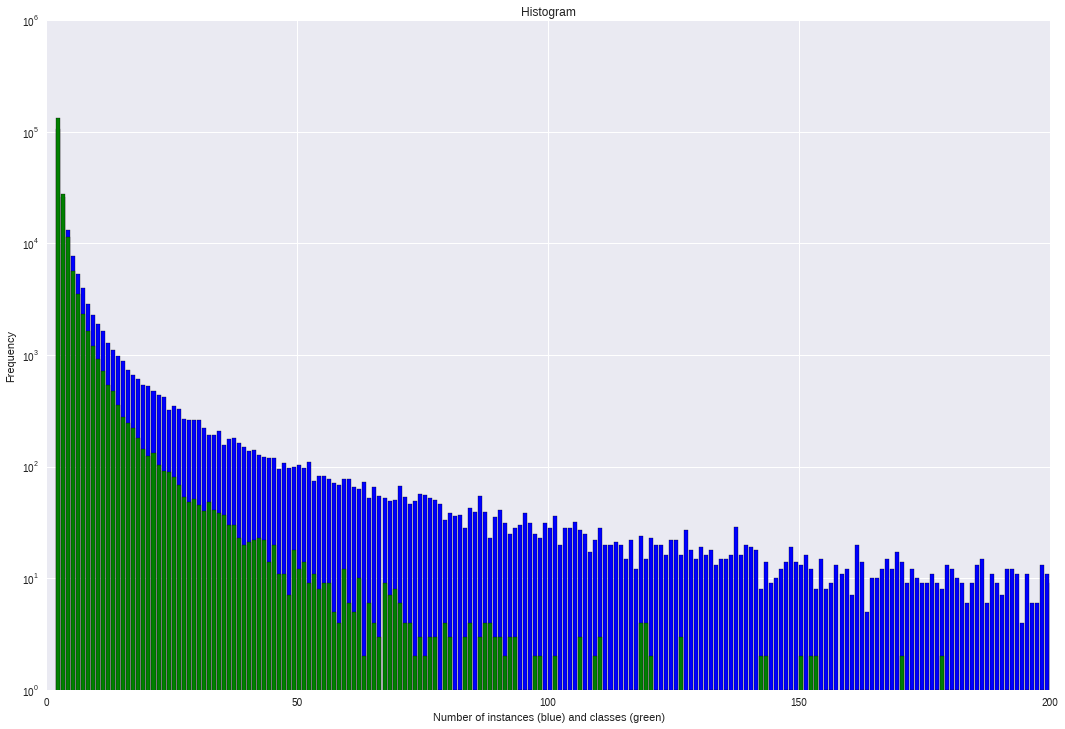
\includegraphics[width=90.00mm]{classifierhistogram.png}
\caption{Histogram showing the distribution of the number of instances (blue)
and number of classes (green) in the classifier experts for IWSLT 2012 TED,
Dutch to English (logarithmic).}
\label{fig:histogram}
\end{center}
\end{figure}

Most of the tables in Section~\ref{sec:results1} list results for both classifier
types.  We find the classifier experts outperforming the monolithic classifier
for Chinese-English (Table~\ref{tab:iwslt2006zhen} (for all context sizes except
\texttt{l3r3}), for  IWSTL 2012 TED Dutch-English (Table~\ref{tab:iwslt2012},
mostly below baseline), Europarl250k Dutch-English
(Table~\ref{tab:europarl250k}, mostly below baseline), and Frisian-Dutch
(Table~\ref{tab:fa2}, all below baseline).

These results suggest that the classifier experts perform better than the
monolithic classifier. When looking at the two 250,000 instance samples of
JRC-Acquis (Table~\ref{tab:jrc250k}), we see a conflicting image. One sample
confirms our hypothesis that the classifier experts are better, whereas in the
other the monolithic classifier has the upper-hand. Moreover, when we look at
the EMEA data (Table~\ref{tab:emea}), where we had the most significant gains
above baseline, we find the monolithic system strongest. 

Despite the results not being unanimous, the case for the classifier experts is
strong and can be motivated by the fact that feature weights are computed on a
per-source-phrase basis, rather than on the aggregation of all. It can be
considered as a kind of optimisation step, in absence of classifier parameter
optimisation and explicit variable context selection (see Section~\ref{sec:paropt}). The
disadvantage is that such systems may be more prone to overfitting, which might
well be the case in the EMEA experiment.


\subsection{Weighting methods and score analysis}
\label{sec:weighting}

Two weighting methods have been implemented: the \emph{append} method, adding
$p(t|s,C)$ as an extra score to the score vector, and the \emph{replace}
method, which replaces the existing $p(t|s)$ score with $p(t|s,C)$. Most
experiments have been conducted with the \emph{replace} method, as it is the
simplest one. For EMEA (Table~\ref{tab:emea}) and JRC
(Table~\ref{tab:jrc250k}), the \emph{append} method was tested as well.

Comparing the two weighting methods, however, is far from trivial. When a
discrepancy is found between a run with the replace method (4 scores) and the
run with the append method (5 scores), we can not simply ascribe such a
difference to the extra score, but must take into account that the very act of
adding a score shifts the weights for the score vector, even if uniformly
distributed. Any shift may likely affect the outcome. This
motivation is also the reason we included a separate baseline for the append
method in the tables in which we reported it. Moreover, it explains why we can
not just apply the results of the parameter optimisation of the replace method
to the append method.

Tables~\ref{tab:emea} (EMEA) and \ref{tab:jrc250k} (JRC) have been run without
parameter optimisation. Even without context information, the baselines for the
append method score better than those for the replace method. Effectively, the
append method's baseline is simply a version with a double feature and
functionally equivalent to just assigning double weight to the feature.

A comparison is complicated by the fact that the $p(t|s,C)$ score is often simply
equal to the $p(t|s)$ score, by definition so for any source phrases for which no
classifier was needed, due to not being ambiguous in translation or context. 

We can therefore not draw any satisfactory conclusions on the merit of the
\emph{append} method versus the \emph{replace} method, given the experiments we
conducted. We can, however, use the two different scoring methods to provide
insight into the classifier results. How often does the classifier assign a
$p(t|s,C)$ that significantly differs from $p(t|s)$? And how often are they
completely identical?  Such an analysis has been conducted on the test data of
the JRC-Acquis corpus, from English to Spanish. This is shown in
Figure~\ref{fig:scoredifference}.

For each occurrence of each source phrase in the test-data, we gathered all
possible translations and computed $\frac{p(t|s,C)}{p(t|s)}$. This ratio
expresses the difference between the context-informed translation probability
and the non-context informed one. A value of one indicates there is no
difference whatsoever, this includes all source phrases where either
translation or context are unambiguous. An outlier point can
be observed at this point, covering $9\%$ of phrase-pairs. The right hand side
of the graph ($>1$) is of most interest; it covers the phrase pairs to which
the classifier assigns a higher probability. No less than $75\%$ of the phrase
pairs are in this region.

\begin{figure}
\begin{center}
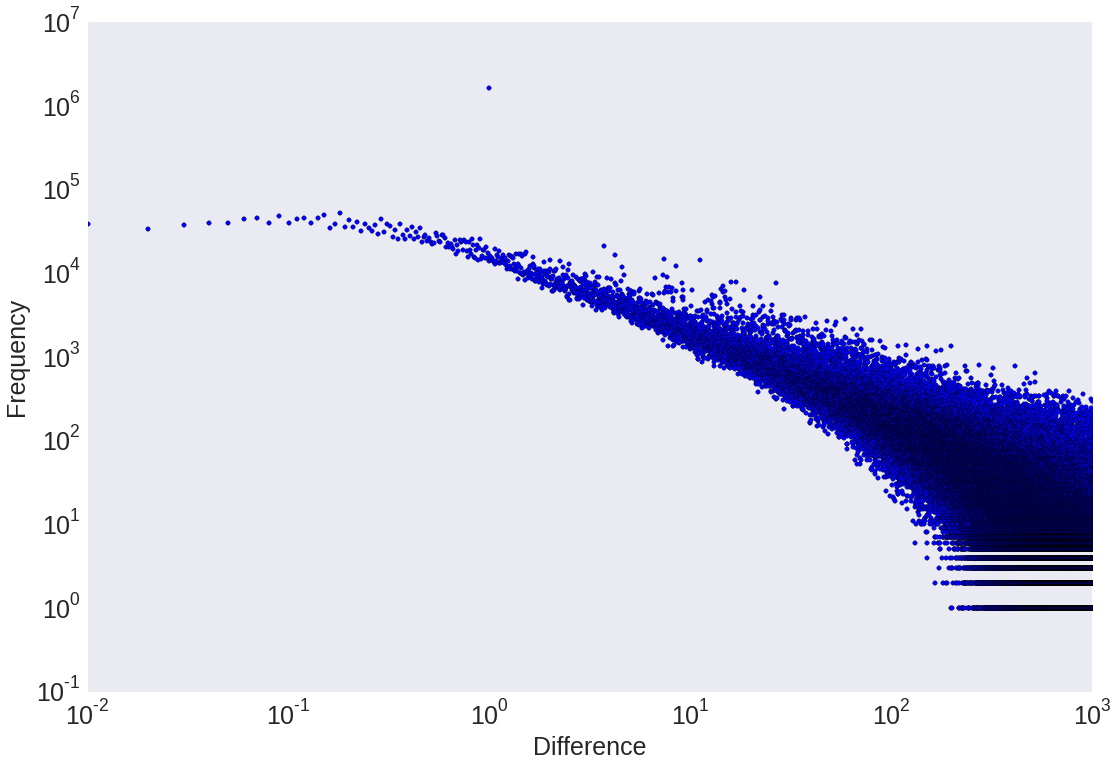
\includegraphics[width=90.00mm]{scoredifference.png}
\caption{Scatter plot (logarithmic scale) showing the ratio
$\frac{p(t|s,C)}{p(t|s)}$ on the  JRC250k English to Spanish test set, illustrating the difference between the classifier score and the original SMT score.}
\label{fig:scoredifference}
\end{center}
\end{figure}


\subsection{Qualitative analysis}
\label{sec:qualanal}

In this section we take a closer look at the translations themselves and see if
we can discern patterns that can tell us what the effect of source-side context
information is and when it pays off.

We zoom in on the corpus that performed best, the EMEA corpus -- English to
Spanish, one million sentence pairs. We compare the context-informed
\texttt{l1r1} system with the non-context informed baseline to assess the
impact of the context information. Out of $5,000$ sentences in the test set,
$3,863$ ($77\%$) are translated identically. This high number again shows that
it is difficult to make a difference. Nevertheless, $22\%$ differs and results
in a net gain in translation performance, as seen in Table~\ref{tab:emea}.

The next few examples will show some comparisons in which the context-informed
improves over the baseline. 

Example~\ref{ex:QAsynonym} shows three examples of the selection of a better
translation given the context, matching with the reference translation, even
though the baseline translation could be considered correct as well. This is
the most common type of difference. Example~\ref{ex:QAdrop} shows the dropping
of a word. Example~\ref{ex:QAgrammar} shows selection of a grammatically better
phrase in the context.


\begin{exe}
\footnotesize
\ex \textbf{Baseline:} El cambio continuo del lugar de inyección dentro de \underline{un área} determinada puede ayudar a \\
\textbf{l1r1:} El cambio continuo del lugar de inyección dentro de \underline{una región} determinada puede ayudar a \\
\textbf{Reference:} La contínua rotación de los puntos de inyección dentro de \underline{una región} determinada puede ayudar a reducir o prevenir estas reacciones \\
\noindent\makebox[\linewidth]{\rule{\linewidth}{0.4pt}}
\textbf{Baseline:} Baraclude reduce la cantidad de virus en su \underline{cuerpo} y mejora el estado del hígado . \\
\textbf{l1r1:} Baraclude reduce la cantidad de virus en su \underline{organismo} y mejora el estado del hígado  \\
\textbf{Reference:} Baraclude reduce la cantidad de virus en su \underline{organismo} y mejora el estado del hígado .
\\ 
\noindent\makebox[\linewidth]{\rule{\linewidth}{0.4pt}}
\textbf{Baseline:} Como consecuencia , el fenilbutirato de sodio , reduce \underline{los niveles plasmáticos} de amonio y glutamina en pacientes con trastornos del ciclo de la urea . \\
\textbf{l1r1:} Como consecuencia , el fenilbutirato de sodio reduce \underline{las concentraciones plasmáticas elevadas} de amonio y glutamina en pacientes con trastornos del ciclo de la urea .  \\
\textbf{Reference:} Como consecuencia , el fenilbutirato de sodio reduce \underline{las concentraciones plasmáticas elevadas} de amoníaco y glutamina en pacientes con trastornos del ciclo de la urea .
\label{ex:QAsynonym}
\end{exe}

\begin{exe}
\footnotesize
\ex \textbf{Baseline:} \underline{Los estudios} en animales , no pueden excluir el desarrollo potencial de toxicidad ( ver sección 5.3 ) . \\
\textbf{l1r1:} \underline{Estudios} en animales , no pueden excluir el desarrollo potencial de toxicidad ( ver sección 5.3 ) . \\
\textbf{Reference:} \underline{Estudios} en animales , no pueden excluir el desarrollo potencial de toxicidad ( ver sección 5.3 ) .
\label{ex:QAdrop}
\end{exe}

\begin{exe}
\footnotesize
\ex \textbf{Baseline:} Las reacciones adversas \underline{consideradas relacionadas} con el uso de Agenerase son síntomas gastrointestinales , erupción y parestesia oral / peri-oral . \\
\textbf{l1r1:}  Las reacciones adversas \underline{que se consideran relacionadas} con el uso de Agenerase son síntomas gastrointestinales , erupción y parestesia oral / \\
\textbf{Reference:} Las reacciones adversas \underline{que se consideran relacionadas} con el uso de Agenerase son síntomas gastrointestinales , erupción y parestesia oral / perioral . \\ \\
\label{ex:QAgrammar}
\end{exe}

In addition to the positive examples, there are also neutral and negative
examples. In example~\ref{ex:QAneutral}, all translations can technically be
considered correct and convey the same message with different nuances; a
different construction is chosen. Example~\ref{ex:QAnegative} shows the
inverse situation of example~\ref{ex:QAsynonym}; a different synonym was chosen
but it does not match with the reference translation. This too is a common
pattern in the data. This raises the question whether the impact of
context-information would not be lower if the test set would have contained
multiple reference translations. Such data unfortunately is hard to come by and
was not available in this study.

\begin{exe}
\footnotesize
\ex \textbf{Baseline:} Asegúrese de que el polvo \underline{esté completamente disuelto} . \\
\textbf{l1r1:} Asegúrese de que el polvo \underline{se disuelva completamente} .  \\
\textbf{Reference:} Asegúrese de que el polvo \underline{se ha disuelto completamente} .
\label{ex:QAneutral}
\end{exe}

\begin{exe}
\footnotesize
\ex \textbf{Baseline:} Los pacientes \underline{se asignaron aleatoriamente} a recibir 500 $\mu$ g de Aranesp una vez cada tres semanas o 2,25 $\mu$ g / kg una vez a la semana . \\
\textbf{l1r1:} Los pacientes \underline{fueron aleatorizados} a recibir 500 $\mu$ g de Aranesp una vez cada tres semanas o 2,25 $\mu$ g / kg una vez a la semana . \\
\textbf{Reference:} Los pacientes \underline{se asignaron aleatoriamente} a recibir 500 $\mu$ g de Aranesp una vez cada tres semanas o 2,25 $\mu$ g / kg una vez a la semana .
\label{ex:QAnegative}
\end{exe}


\section{Conclusions and Discussion} 

We have conducted numerous experiments to assess whether surface-form
source-side context information, i.e. without the use of any explicit
linguistic features that require supervised parsers or taggers, can improve
translation quality. Memory-based classifiers were used, and integrated in an
SMT framework, following techniques commonly employed in WSD. Different
classifier types, context sizes, and score weighting methods, have been
researched. Parameter optimisation was conducted on the decoder parameters for
various experiments. Optimisation of classifier parameters and feature
selection was omitted in order to contain the computational complexity of the
problem, and considering experiences in prior research.

Various distinct corpora and language pairs have been employed for the
experiments, this in order to ensure that conclusions are of a generic
enough nature rather than incidental artifacts. The results of the
experiments, however, were still often in contrast with one another;
there was a high degree of variability between the corpora and
language pairs. Positive results were attained on EMEA, for both
English to Spanish and English to Dutch, JRC-Acquis (English to
Spanish) and IWSLT 2006 (English to Chinese).  Especially the former
two are highly formulaic corpora, and the touristic ``how to'' domain of
the IWSLT 2006 data has formulaic aspects as well, leading us to be
cautiously optimistic source-side context does have merit under
certain constraints.

Finding these precise constraints, however, proved elusive. We hypothesised that
source-side context information may contribute more when translating to a
morphologically more complex language, but this was empirically refuted.
An alternative hypothesis was that a certain quality of translation had to
be reached before the source-side context can make an impact. This hypothesis
could not be confirmed on Dutch-Frisian data, and is at odds with the positive
results on IWSLT 2006 English-Chinese, which had relatively little data and low
scores.

In this study, we effectively replicated and expanded upon the part of the work
of \cite{Stroppa+07} and \cite{Rejwanul+11} that does not depend on further
linguistic information. Except for the aforementioned formulaic data sets most
results were below baseline. Inclusion of surface-form source-side context
information is clearly not the most obvious road for the improvement of MT
quality. It is likely that improvement can be more easily achieved through for
example optimisation of the target-side language model.

In this final discussion we would like to focus on why the results of our study
overall do not exceed above the baseline.  There may be an explanation for this
if we look at the interplay between the SMT decoder and the classifiers. The
classifier instances are generated with the phrase-translation table as input,
looking up the context in the corpus. There will therefore never be phrases in
the classifier training data that do not occur in the classifier. If we have a
classifier training instance $(s,C) \mapsto t$, i.e.  a source phrase $s$ with
context $C$ and mapping to translation $t$, and $C$ is a context that occurs
multiple times in the corpus, then there is often a source fragment $s'$ in the
phrase-translation table that is the conjunction of $s$ and $C$, and which maps
to a $t'$ of which $t$ is at least a substring. In other words, if a context
for a source phrase is prevalent enough in the data, then this context may be
an integral part of a larger source phrase. Only if the context is not
prevalent at all, then no such $s'$ exists, in which case one may also posit
that the context is less likely to occur in test data and the training instance
is therefore considered fairly weak.  It is thus likely that the context
information we try to \emph{explicitly} model, is often already
\emph{implicitly} available to the decoder.  Rather than considering a source
phrase in context, the decoder may thus opt to choose to include the context as
integral part of the phrase.  The target-language model already plays an
important role here, as it encourages the decoder to choose translation options
that fit well together. Source-side context modelling, without additional
linguistic features, seems to only have something to offer for highly formulaic
corpora. 


\bibliographystyle{spbasic}
\bibliography{sourcecontextinsmt}




\end{document}
